\documentclass{article}
\usepackage[utf8]{inputenc}
\usepackage[russian]{babel}
\usepackage{enumitem}

\title{Design document}
\date{November 2024}

\begin{document}

\section{Введение}
Организация содержимого документа соответствует принятому стандарту оформления диздока.
Авторы: Береснев Вадим, Варакин Владислав, Громова Дарья, Демина Дарья, Мальцев Владислав, Попов Роман.

\section{Концепция}

\subsection{Введение}
Игра "Путешествие Лили" — это увлекательный платформер для детей и подростков, в котором игроки помогают любопытной лягушке Лили исследовать мир, собирая насекомых и избегая врагов на протяжении различных уровней, включая захватывающие битвы с боссами. Игрокам предстоит развивать ловкость и стратегическое мышление, чтобы преодолевать препятствия и открывать новые локации, узнавая интересные факты о фауне и экосистемах разных мест.

\subsection{Жанр и аудитория}
\begin{itemize}
    \item \textbf{Жанр:} платформер с элементами экшена и приключения
    \item \textbf{Возрастная группа:} 6+. Игра подходит для широкой аудитории.
    \item \textbf{Другие сведения о позиционировании игры:} образовательная и познавательная наклонность
\end{itemize}

\subsection{Основные особенности игры}
Попадая в новой мир, лягушка знакомится с другими лягушками, которые обитают в соответствующем биоме. Каждый мир представляет собой существующую климатическую зону, а местные лягушки, насекомые, птицы и змеи соответствуют действительно живущим в данных климатических зонах животным. При открытии нового мира игроку показывается справочная информация о лягушке, насекомых, птицах и змеях, которых игрок встретит в этом мире (название, внешний вид в реальном мире, ареал обитания, особенности, интересные факты). Таким образом, игра интересна не только процессом геймплея, но и познавательной стороной.

\subsection{Описание игры}
Игрок управляет лягушкой Лили, цель которой - увидеть мир, состоящий из 5 локаций. Для того чтобы попасть в другую локацию, необходимо договориться с животным, которое может перенести игрока (птица\крот и.т.д). Животное попросит трофей, получив который она будет готова перенести лягушку. На каждой локации будет 6 уровней, последний из которых – уникальная битва с боссом. На первых пяти уровнях игра представляет собой платформер, с препятствиями, врагами и насекомыми, которых лягушка может собирать. Для этого необходимо прицелится и выстрелить языком, точно попав по цели. Игроку необходимо успеть дойти до конца уровня за отведенное время. Уровень перезапускается если Лили получает урон или заканчивается время. За количество собранных насекомых, после каждого уровня игрок получит от одной до трех звезд. Перед уровнем с боссом будет возможность потратить накопленные звезды на различные улучшения (урон от удара языком, расходник защищающий от одного удара босса, и.т.д). Битва с боссом будет отличаться специальным условием победы, уникальным для каждого. После победы над боссом игрок будет получать трофей, необходимый для попадания на следующую локацию.


\subsection{Предпосылки создания}

\subsubsection{Общие тенденции рынка}

Рынок игр платформеров и адвенчур остается стабильным и востребованным, особенно в сегменте инди-игр. Платформеры, такие как \textit{Hollow Knight}, \textit{Celeste} и \textit{Ori and the Blind Forest}, демонстрируют устойчивый интерес аудитории благодаря сочетанию увлекательного геймплея, интересных персонажей и визуально привлекательных миров. Уникальная механика игры, где игрок управляет лягушкой с использованием языка для взаимодействия с окружением и борьбы, добавляет свежесть в жанр. Элементы сбора ресурсов и система звезд обеспечивают высокую реиграбельность, что важно для привлечения игроков к повторному прохождению уровней. 

Кроме того, комбинация платформера и адвенчуры, наряду с яркой, дружелюбной атмосферой, делает игру привлекательной для широкой аудитории, включая детей, подростков и казуальных геймеров, что соответствует современным трендам.

\subsubsection{Вопросы лицензирования}

Нет лицензии (пока что)

\subsection{Технические требования}
\begin{center}
\begin{tabular}{ c | c | c }
 & Минимальные технические & Рекомендуемые технические \\ 
 & требования & требования \\ [2ex]
 Операционная система & Windows 10 & Windows 10, 11 \\ [2ex] 
 Процессор & AMD Ryzen 3 1200 & AMD Ryzen 3 4100 \\  
 & Intel i3-8100 & Intel i3-12100 \\ [2ex]
 ОЗУ & 4 GB & 8 GB \\ [2ex]
 CD-ROM привод & Не требуется & Не требуется \\ [2ex]
 Свободное место на HDD & 8 Gb & 8 Gb \\ [2ex]
 Видео карта & Nvidia GTX 950 & Nvidia GTX 970 \\
 & AMD Radeon RX 560 & AMD Radeon RX 580 \\ [2ex]
 Звуковая карта & Достаточно встроенной & Достаточно встроенной \\
 & в материнскую плату & в материнскую плату \\
 & звуковой карты & звуковой карты \\ [2ex]
 Управление & Клавиатура + мышь & Клавиатура + мышь \\ [2ex]
 DirectX & 11 & 11 \\
\end{tabular}
\end{center}

\section{Функциональная спецификация}

\subsection{Принципы игры}

\subsubsection{Суть игрового процесса}

Основа геймплея - передвижение по платформам. \\
Каждая игровая локация содержит пять обычных уровней и один уровень с боссом. \\
Время на прохождение обычного уровня ограничено. Чтобы его пройти, нужно успеть добраться до контрольной точки. На уровне игрок встретит различных врагов (змей, птиц) и ловушки (зыбучие пески, острые камни и т.д), которых он должен мастерски избегать, чтобы не умереть, а также насекомых, которых он может есть, используя язык лягушки. Если лягушка погибнет или закончится время, уровень будет считаться непройденным. При успешном прохождении уровня за съеденных насекомых игрок получит звезды (если игрок соберет 75-100\% насекомых, то он получит 3 звезды, если 50-74\% — 2 звезды, 25-49\% — 1 звезду, 0-24\% — 0 звезд), которые он сможет использовать для приобретения улучшений перед схваткой с боссом (двойной урон, увеличивающий урон языка лягушки с 1 единицы до 2 единиц, щит, защищающий лягушку от одной атаки босса, дополнительное время и т.д).
Каждый уровень с боссом уникален. Описание некоторых из них:
\begin{itemize}
    \item 1. Цель игрока: продержаться определенное время, уклоняясь от атак босса.
    \item 2. Цель игрока: за определенное время успеть убить перемещающегося по уровню босса, используя язык лягушки, не попав при этом в ловушки.
    \item 3. Бесконечный уровень, игрока преследует босс, скорость которого постоянно увеличивается. Цель игрока: покинуть логово босса.
\end{itemize}

При прохождении уровня с боссом игрок получит трофей, который откроет ему следующую локацию.

\subsubsection{Ход игры и сюжет}

Типичный «сеанс» игры: Для продвижения по сюжету игрок проходит уровни открытой для него на данный момент локации. В процессе прохождения они используют возможности Лягушки Лили прыгать, бегать, плавать, стрелять языком для того, чтобы избегать врагов, ловушки и есть насекомых. Если игроку удалось помочь персонажу не погибнуть и добраться до контрольной точки в срок, для него открывается новый уровень. Так пройдя все уровни, перед испытанием с боссом игрок может на собранные звёзды приобрести улучшения для лягушки.

Сюжет: Лягушка по имени Лили прожила всю свою жизнь на родном болоте и ни разу не покидала его границы. Однако, несмотря на свою привычную среду обитания, в глубине души она всегда испытывала сильное желание и стремление узнать, как живут другие существа за пределами её дома. Каждый раз, когда она наблюдала за птицами, парящими в небесах и свободно исследующими мир, в её сердце возникали горечь и зависть. Ей хотелось увидеть все те удивительные места, о которых она только слышала от других обитателей болота. И вот однажды Лили пришла к идее, которая могла бы помочь ей осуществить свою мечту о путешествиях. Она решила заключить сделку с птицами: она добудет для них необходимый трофей, а взамен они помогут ей покинуть болото и перенесут её в неизведанные земли. Как только условия уговора лягушка выполнила, успешно пройдя все 6 уровней локации, птицы с радостью помогли ей перебраться в новую местность, где она познакомилась с местными представителями фауны и узнала об их особенностях. Так, проходя уровни, побеждая боссов и доставая трофеи для сделок с животными/птицами, Лягушка Лили путешествует по миру, посетив множество различных мест: от родного болота до лиственного леса, затем джунглей, пустыни и даже гор.

\subsection{Физическая модель}
Описание физической модели игрового мира, ее законов и их отображения в игру. 

\subsubsection{Перемещения}
Движение персонажа подчиняется классическим законам механики: 
\begin{itemize}
    \item Перемещение происходит по двум осям (X, Y) в системе координат игрового мира.
    \item Лягушка может прыгать, бегать и плавать под водой. Параметры, такие как высота и длина прыжка, зависят от скорости и продолжительности нажатия кнопки прыжка.
    \item Эффект гравитации воздействует на персонажа, что создает реалистичное ускорение вниз. Используется формула $a = g$, где $g = 9.8 \frac{м}{с^2}$, с возможными вариациями для уникальных миров.
\end{itemize}

\subsubsection{Боевые действия}
Боевая система включает следующие элементы:
\begin{itemize}
    \item Лягушка Лили атакует языком, выстреливая его в направлении цели. Дальность и скорость языка определяются формулой $v = v_0 + a \cdot t$, где $v_0$ — начальная скорость, $a$ — ускорение.
    \item Враги имеют уникальные зоны уязвимости и атакуют игрока по заданным паттернам.
    \item Урон врагу рассчитывается по формуле $D = P \cdot F_{crit}$, где $P$ — базовый урон, а $F_{crit}$ — множитель критического удара.
\end{itemize}

\subsubsection{Другие важные моменты}
\begin{itemize}
    \item \textbf{Столкновения:} Логика столкновений использует прямоугольные или круговые хитбоксы для определения взаимодействия между объектами.
    \item \textbf{Повреждения:} Игрок получает урон, если хитбокс врага касается Лили. Также возможна симуляция рикошета при столкновении с твердыми поверхностями.
    \item \textbf{Сопротивление среды:} В некоторых уровнях (например, под водой) на движения Лили влияет сопротивление, моделируемое по формуле $F = -k \cdot v$, где $k$ — коэффициент сопротивления, $v$ — скорость.
    \item \textbf{Моделирование разрушений:} Некоторые элементы игрового окружения могут разрушаться под воздействием игрока или врагов, например, ветки, которые ломаются под весом персонажа.
\end{itemize}

\subsection{Персонаж игрока}

\begin{wrapfigure}{r}{0.4\textwidth}
    \centering
    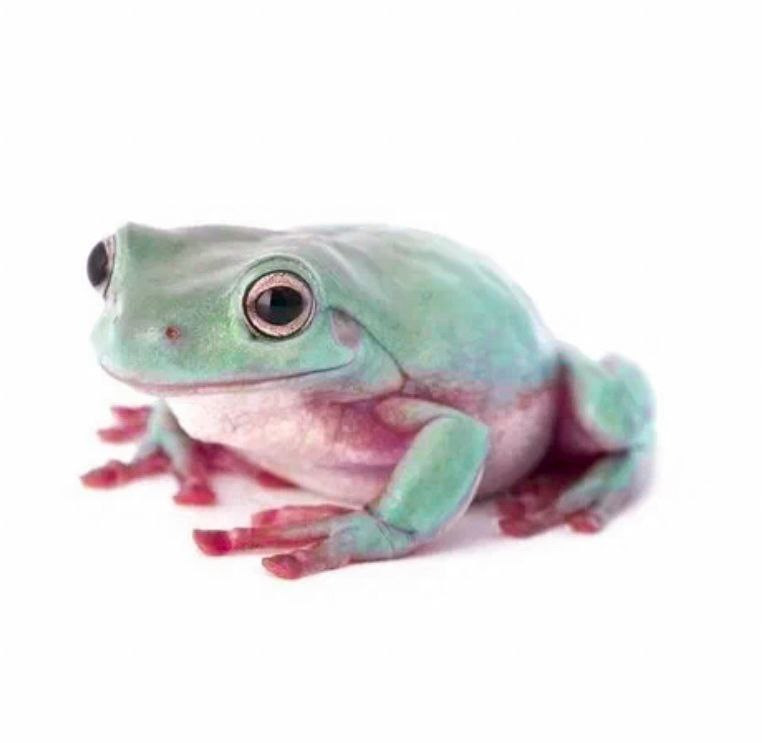
\includegraphics[width=0.4\textwidth]{https://raw.githubusercontent.com/vadyukkha/design_document_unity_game/refs/heads/main/pictures/photo_2024-12-01_22-21-33.jpg} 
    \caption{\textit {Референс главного персонажа}}
    \label{fig:example}
\end{wrapfigure} 
Аватар игрока (лягушка) представляет собой частично реалистичную лягушку. Окрас лягушки соответствует виду коралловопалая литория (рис. 1).  Лягушка передвигается прыжками, в  момент прыжка персонаж повёрнут в профиль. Профильная сторона детально прорисована в соответствии с референсным изображением. Механика прыжка и высовывания языка соответствуют действительной механике упомянутых движений коралловопалой литории. Исключением из реалистичности образа персонажа является механика передвижения под водой, высота и длина прыжка, вариация длины языка в большую сторону и наличие эмоций на морде. Соответствующие эмоции (радость, грусть) проявляются при успешном или неудачном прохождении уровня.

\subsection{Элементы игры}
\subsubsection{Персонажи}

\begin{enumerate}
\item Главный герой - Лягушка Лили
    \begin{itemize}
     \item \textbf{Цель:} главный герой игры, которым управляет игрок. Она путешествует по миру, исследуя биомы, взаимодействуя с неигровыми персонажами, собирая насекомых и сражаясь с боссами.
     \item \textbf{Влияние на игровой мир:} Лили – аватар игрока.
     \item \textbf{Жизни:} по умолчанию одна жизнь.
     \item \textbf{Скорость:} средняя, может быть улучшена временными бонусами.
     \item \textbf{Cпособности:}
     \begin{itemize}
            \item Прыжки: используются для обхода ловушек, врагов и перехода по платформам.
            \item Удар языком: используется для сбора насекомых и нанесения урона врагам.
            \item Полет на языке: лягушка цепляется языком за точку и летит, перемещаясь по платформам
            \item Плавание
     \end {itemize}
     \end{itemize}
\end{enumerate}

\subsubsection{Локации}
\begin{enumerate}
    \item Биомы
    \begin{itemize}
     \item \textbf{Цель:} каждый биом — это уникальная игровая локация, связанная с определенным климатом.
     \item \textbf{Влияние на игровой мир:} служит местом действия самой игры, знакомит игрока с разными климатами и животными.
     \item \textbf{Особенности:}
        \begin{itemize}
            \item Болота - родной мир Лили, влажные условия, сложные платформы. 
            \item Леса
            \item Джунгли – экзотическая флора и фауна. БОльшая динамичность.
            \item Пустыни - жаркая погода, песчаные бури и змеи.
            \item Горы - большая высота, ветрено.
            
        \end{itemize}
    \end{itemize}
    
    \item Ловушки
    \begin{itemize}
     \item \textbf{Цель:} элементы уровня, создающие дополнительные трудности для игрока. Они требуют осторожности, ловкости и умения адаптироваться к ситуации.
     \item \textbf{Влияние на игровой мир:} усиливают атмосферу каждой локации, делая ее уникальной, и заставляют игрока исследовать уровни внимательнее.
     \item \textbf{Механики взаимодействия:} некоторые ловушки можно обойти, другие требуют быстрого реагирования.Можно использовать ловушки против врагов (например, заманить их к обвалу)
     \item \textbf{Уникальность:} каждая локация имеет свои особенные ловушки.
     \item \textbf{Классификация ловушек:}
     \begin{itemize}
            \item Типы ловушек:
                \begin{itemize}
                    \item Статичные: просто расположены в локации (к примеру, ямы или прочие естественные преграды)
                    \item Динамичные: препятствия, перемещающиеся по заданной траектории или перемещающие игрока (качающиеся бревна или потоки воды)
                \end{itemize}
            \item Уровень сложности:
                \begin{itemize}
                    \item с небольшими негативными эффектами (например, трясина – только замедляет или не дает прыгать).
                    \item смертельные (например, пропасти или обвалы – моментальная потеря жизни).
                \end{itemize}
     \end {itemize}
     \end{itemize}

    \item Насекомые
    \begin{itemize}
     \item \textbf{Цель:}  насекомые – игровая валюта. Их сбор приносит очки, а вследствие звезды, которые можно потратить на улучшения и расходные материалы 
     \item \textbf{Влияние на игровой мир:} стимулирует игроков перепроходить уровни ради большего числа очков.
     \item \textbf{Награды за сбор:} в зависимости от редкости и сложности поимки, игрок получает соответственное количество очков
     \item \textbf{Классификация:}
            \begin{itemize}
                \item Статичные - стоят на месте, легчайшая цель.
                \item Медленные - летают низко и медленно, легко поймать.
                \item Быстрые - требует точного прицеливания и реакции, сложная цель.
                \item Редкие – могут улетать/пропадать с уровня со временем, самая трудная цель.
            \end{itemize}
     \end {itemize}

    \item Магазин с улучшениями и расходными материалами
    \begin{itemize}
     \item \textbf{Цель:} магазин служит для улучшения лягушки или покупки расходных материалов для более легкого прохождения. 
     \item \textbf{Влияние на игровой мир:} стимулирует игроков собирать больше звезд и насекомых, награждая за выполнение задач и исследование уровней.
     \item \textbf{Местоположение:} магазин доступен перед каждым боссом
     \item \textbf{Виды товаров:}
     \begin{itemize}
            \item Расходные материалы - разовые бонусы (например, дополнительная жизнь или усиленные атаки на время)
            \item Улучшения - постоянные бонусы (например, увеличение силы атаки, скорости или прыгучести) 
     \end {itemize}
     \end{itemize}


\end{enumerate}

\end{document}
